\par\addvspace{12pt}\Needspace{9\baselineskip}

\section{导数}

% ITEM: calculus-example-001
\solutionitem{calculus-example-001}{例5.1}
某质点的位置为\(s(t)=t^2+2t\)。分别计算从\(t=1\)到\(t=1+h\)及从\(t=2\)到\(t=2+h\)的平均速度。令\(h\)分别取正数和负数，解释所比较的时间范围。
\solutionanswer
两段平均速度分别为\(4+h\)、\(6+h\)，例如第一段由\([s(1+h)-s(1)]/h=[4h+h^2]/h\)得到。\(h>0\)考察基准时刻之后，\(h<0\)考察之前；后一情形的时间增量与位移都按从基准时刻到\(t+h\)的方向计算，所得仍是相应时间段的平均速度。令\(h\to0\)，分别趋于\(4,6\)。


% ITEM: calculus-example-002
\solutionitem{calculus-example-002}{例5.2}
用定义求\(f(x)=x^3\)在\(x_0\)处的导数。再设\(g(x)=\sqrt{x}\)，用有理化求\(g'(x_0)\)，其中\(x_0>0\)。
\solutionanswer
立方函数的差商为\(3x_0^2+3x_0h+h^2\)，趋于\(3x_0^2\)。平方根有理化后为
\[
 \frac{\sqrt{x_0+h}-\sqrt{x_0}}h
 =\frac1{\sqrt{x_0+h}+\sqrt{x_0}}\longrightarrow\frac1{2\sqrt{x_0}}.
\]
所以\(f'(x_0)=3x_0^2,g'(x_0)=1/(2\sqrt{x_0})\)。


% ITEM: calculus-exercise-01-01
\solutionitem{calculus-exercise-01-01}{习题5.1（1）}
用定义求\(f(x)=1/x\)在\(x_0\ne0\)处的导数。
\solutionanswer
\(\dfrac{1/(x_0+h)-1/x_0}{h}=-\dfrac1{x_0(x_0+h)}\to-1/x_0^2\)，故\(f'(x_0)=-1/x_0^2\)。


% ITEM: calculus-exercise-01-02
\solutionitem{calculus-exercise-01-02}{习题5.1（2）}
设\(f(x)=x|x|\)。判断它在原点是否可导，并与\(|x|\)比较。
\solutionanswer
在原点的差商为\(h|h|/h=|h|\to0\)，所以可导且导数为\(0\)。\(|x|\)的差商为\(|h|/h\)，左右极限不同，故不可导。两者都连续，但乘上一个\(x\)使前者的差商振幅趋零。


% ITEM: calculus-exercise-01-03
\solutionitem{calculus-exercise-01-03}{习题5.1（3）}
设\(f(0)=0\)，\(x\ne0\)时\(f(x)=x\sin(1/x)\)。判断\(f\)在原点是否连续、可导。
\solutionanswer
\(|x\sin(1/x)|\le|x|\to0\)，故在原点连续；差商为\(\sin(1/h)\)，沿\(h_n=1/(\pi/2+2n\pi)\)、\(k_n=1/(3\pi/2+2n\pi)\)分别为\(1,-1\)，故不可导。


% ITEM: calculus-example-003
\solutionitem{calculus-example-003}{例5.3}
求\(f(x)=|x|\)的导函数及其定义域。已知某函数在\((-1,0)\)上导数为负、在\((0,1)\)上导数为正，试画出可能的原函数图像，并考虑\(x=0\)处的取值是否已被这些信息确定。
\solutionanswer
\(|x|\)的导函数在\(x<0\)时为\(-1\)，在\(x>0\)时为\(1\)，定义域为\(\mathbb R\setminus\{0\}\)。
后一个问题可取\(F(x)=x^2\)（\(x\ne0\)），而\(F(0)\)任意。例如图中取\(F(0)=1\)，两侧导数的符号仍符合要求：
\begin{center}
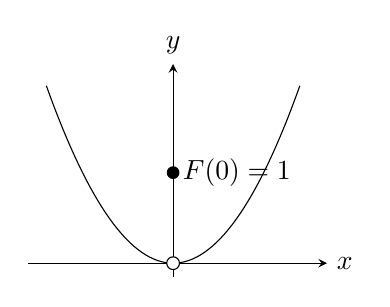
\begin{tikzpicture}[scale=1.15,>=stealth]
\draw[->] (-1.6,0)--(1.7,0) node[right]{$x$};\draw[->] (0,-.15)--(0,2.2) node[above]{$y$};
\draw[domain=-1.4:1.4,samples=65] plot(\x,{\x*\x});\draw[fill=white] (0,0) circle(2pt);\fill (0,1) circle(2pt) node[right]{$F(0)=1$};
\end{tikzpicture}
\end{center}
导数条件没有涉及零点的函数值，不能据此确定它；也不能在尚未给出连续性的情况下把两侧图像强行接起来。


% ITEM: calculus-example-004
\solutionitem{calculus-example-004}{例5.4}
用导数求抛物线\(y=x^2\)在\((1,1)\)处的切线和法线，并用第四章的方法核对。再求\(y=x^3\)在原点的切线。
\solutionanswer
在\((1,1)\)处，导数\(2\)给出切线\(y-1=2(x-1)\)，即\(2x-y=1\)；法线为\(x+2y=3\)。第四章的切线公式\(2x_0x=y+y_0\)在\(x_0=y_0=1\)时也给出\(2x-y=1\)。\(x^3\)在原点的差商为\(h^2\to0\)，切线为\(y=0\)，曲线穿过切线并不影响相切。


% ITEM: calculus-example-005
\solutionitem{calculus-example-005}{例5.5}
（2012年广东卷理科第12题）

求曲线\(y=x^3-x+3\)在点\((1,3)\)处的切线方程。用导数定义确定切线斜率。
\solutionanswer
按定义，在\(x=1\)处的差商为
\[
 \frac{(1+h)^3-(1+h)+3-3}{h}=2+3h+h^2\longrightarrow2.
\]
所以切线为\(y-3=2(x-1)\)，即\(y=2x+1\)。


% ITEM: calculus-exercise-02-01
\solutionitem{calculus-exercise-02-01}{习题5.2（1）}
（2013年大纲卷文科第10题改编）曲线\(y=x^4+ax^2+1\)在点\((-1,a+2)\)处切线的斜率为\(8\)，求\(a\)。用差商极限完成计算。
\solutionanswer
在\(-1\)处的差商展开为\(-4-2a+(6+a)h-4h^2+h^3\)，故切线斜率为\(-4-2a\)。令其等于\(8\)，得\(a=-6\)。


% ITEM: calculus-exercise-02-02
\solutionitem{calculus-exercise-02-02}{习题5.2（2）}
（2012年安徽卷文科第17题第（2）问）设\(f(x)=ax+1/(ax)+b\)，\(a>0\)。若曲线\(y=f(x)\)在点\((1,f(1))\)处的切线方程为\(y=3x/2\)，求\(a,b\)。
\solutionanswer
用差商可得\(f'(1)=a-1/a\)。切线经过\((1,3/2)\)且斜率为\(3/2\)，所以
\[
 a+\frac1a+b=\frac32,\qquad a-\frac1a=\frac32.
\]
第二式解得\(a=2\)或\(-1/2\)，由\(a>0\)取\(a=2\)，继而\(b=-1\)。


% ITEM: calculus-exercise-03-01
\solutionitem{calculus-exercise-03-01}{习题5.3（1）}
用微分近似计算\(\sqrt{4.04}\)，再用上式给出误差上界。
\solutionanswer
在\(x=4\)处用\(dy=h/4\)，取\(h=0.04\)，得\(\sqrt{4.04}\approx2.01\)。由题给精确余项，
\[
 0<2.01-\sqrt{4.04}
 =\frac{0.04^2}{4(\sqrt{4.04}+2)^2}<\frac1{40000}.
\]


% ITEM: calculus-exercise-03-02
\solutionitem{calculus-exercise-03-02}{习题5.3（2）}
对\(f(x)=1/x\)，写出在\(x=1\)处的增量、微分及两者之差。
\solutionanswer
\(\Delta y=1/(1+h)-1=-h/(1+h)\)，微分为\(dy=-h\)，两者之差为\(h^2/(1+h)\)。这一差与\(h\)之比趋零，因而\(-h\)确为线性部分。


% ITEM: calculus-exercise-03-03
\solutionitem{calculus-exercise-03-03}{习题5.3（3）}
设\(f(0)=0\)，\(x\ne0\)时\(f(x)=x^2\sin(1/x)\)。证明\(f\)在原点可导，并写出其在原点的一次近似。
\solutionanswer
差商为\(h\sin(1/h)\to0\)，所以\(f'(0)=0\)。一次近似为\(f(h)\approx0\)，并有\(|f(h)|\le h^2\)，其与\(h\)之比趋零。这并不表示附近函数值恒为零。


% ITEM: calculus-exercise-03-04
\solutionitem{calculus-exercise-03-04}{习题5.3（4）}
设\(f(a)=2\)、\(f'(a)=3\)。分别写出\(f(a+2h)\)与\(f(a-h)\)在\(h\to0\)时的一次近似，并求\(\displaystyle\lim_{h\to0}\frac{f(a+2h)-f(a-h)}h\)。
\solutionanswer
由导数定义的增量表达式，\(f(a+2h)=2+6h+r_1(h)\)、\(f(a-h)=2-3h+r_2(h)\)，其中\(r_i(h)/h\to0\)。相减并除以\(h\)，极限为\(9\)。


% ITEM: calculus-exercise-03-05
\solutionitem{calculus-exercise-03-05}{习题5.3（5）}
圆的半径为\(r>0\)，测量误差为\(h\)。写出面积的实际增量与微分；若半径的相对误差不超过\(1\%\)，估计面积的相对误差，并给出由精确增量得到的上界。
\solutionanswer
\(\Delta S=2\pi rh+\pi h^2\)，\(dS=2\pi rh\)。微分给出的相对误差约为\(2|h|/r\)，故约不超过\(2\%\)。精确式给出
\[
 \frac{|\Delta S|}{\pi r^2}=\left|2\frac hr+\frac{h^2}{r^2}\right|
 \le0.0201=2.01\%,
\]
上界在\(h/r=0.01\)时取得。


% ITEM: calculus-exercise-03-06
\solutionitem{calculus-exercise-03-06}{习题5.3（6）}
设\(f\)在\(a\)处可导，证明\(\bigl(f(a+h)+f(a-h)-2f(a)\bigr)/h\to0\)。这一结论能否推出\(f\)在\(a\)附近为常值？
\solutionanswer
写\(f(a\pm h)=f(a)\pm f'(a)h+r(\pm h)\)，其中\(r(h)/h\to0\)。相加后线性项相消，所得商为\(r(h)/h+r(-h)/h\to0\)。不能推出附近为常值，例如\(f(x)=(x-a)^2\)满足此极限而不恒定。


% ITEM: calculus-exercise-03-07
\solutionitem{calculus-exercise-03-07}{习题5.3（7）}
设\(x<0\)时\(f(x)=ax+b\)，\(x\ge0\)时\(f(x)=x^2\)。分别求\(f\)在原点连续、可导的条件，并用增量的线性部分解释所得结果。
\solutionanswer
右侧函数值趋于\(0=f(0)\)，左侧趋于\(b\)，故连续当且仅当\(b=0\)。此时左差商为\(a\)，右差商为\(h\to0\)，所以可导当且仅当\(a=b=0\)。左右增量的线性部分一致为零，才拼成同一个微分。


% ITEM: calculus-exercise-04-01
\solutionitem{calculus-exercise-04-01}{习题5.4（1） *}
求\(f(x)=x^3\)在\(x_0=1\)处的线性主部，并区分它与切线所给的仿射映射。
\solutionanswer
\((1+h)^3=1+3h+3h^2+h^3\)，故线性主部是增量映射\(L(h)=3h\)；切线给出的仿射映射为\(x\mapsto1+3(x-1)=3x-2\)。前者作用于增量，后者在原坐标中近似函数值。


% ITEM: calculus-exercise-04-02
\solutionitem{calculus-exercise-04-02}{习题5.4（2） *}
对\(r(t)=(t,t^2)\)，求\(t_0=1\)处的向量一次近似，直接检验余项条件。
\solutionanswer
\(r(1+h)=(1,1)+h(1,2)+(0,h^2)\)。向量线性主部为\(h\mapsto h(1,2)\)，余项模与\(|h|\)之比为\(|h|\to0\)。


% ITEM: calculus-exercise-04-03
\solutionitem{calculus-exercise-04-03}{习题5.4（3） *}
回看例5.5，写出函数在\(x=1\)处的线性主部，并求原函数与切线在\(x=1+h\)处的高度差。当\(|h|\le1/10\)时，给出这个误差关于\(h^2\)的上界。
\solutionanswer
该例函数为\(x^3-x+3\)。在\(1\)处有\(f(1+h)=3+2h+3h^2+h^3\)，故线性主部为\(2h\)，高度差为\(h^2(3+h)\)。当\(|h|\le1/10\)时，\(|3h^2+h^3|\le31h^2/10\)。


% ITEM: calculus-exercise-04-04
\solutionitem{calculus-exercise-04-04}{习题5.4（4） *}
对参数曲线\(r(t)=(t^2,t^3)\)，分别求\(t_0=1\)与\(t_0=0\)处的线性主部。零点处的线性主部能否给出非零切向量？再由割线方向判断该处的切线。
\solutionanswer
在\(1\)处有\(r(1+h)=(1,1)+h(2,3)+(h^2,3h^2+h^3)\)，主部为\(h(2,3)\)。在零点\(r(h)=(h^2,h^3)\)，且\(|r(h)|/|h|\to0\)，线性主部为零，不能给出非零切向量；但割线方向可取\((1,h)\)，趋于\((1,0)\)，所以切线仍为\(y=0\)。
\par
